\chapter{Definizione del progetto}
\setcounter{section}{1}
\item
\subsection{Architettura del progetto}
\subsubsection{Concetto Provider/Subscriber}
Il modello di \textit{provider/subscriber} definisce un flusso unidirezionale di informazioni da un oggetto \textit{provider} a un numero qualsiasi di oggetti \textit{subscribers}. Il concetto \`{e} che il \textit{provider}, anche chiamato \textit{publish}, ha informazioni o eventi utili che devono essere comunicati ad altri oggetti, ovvero tutti i suoi \textit{subscriber}, che useranno tali informazioni per eseguire azioni aggiuntive o rimanere sincronizzati con il fornitore. 

\begin{figure}[htbp]
\centering
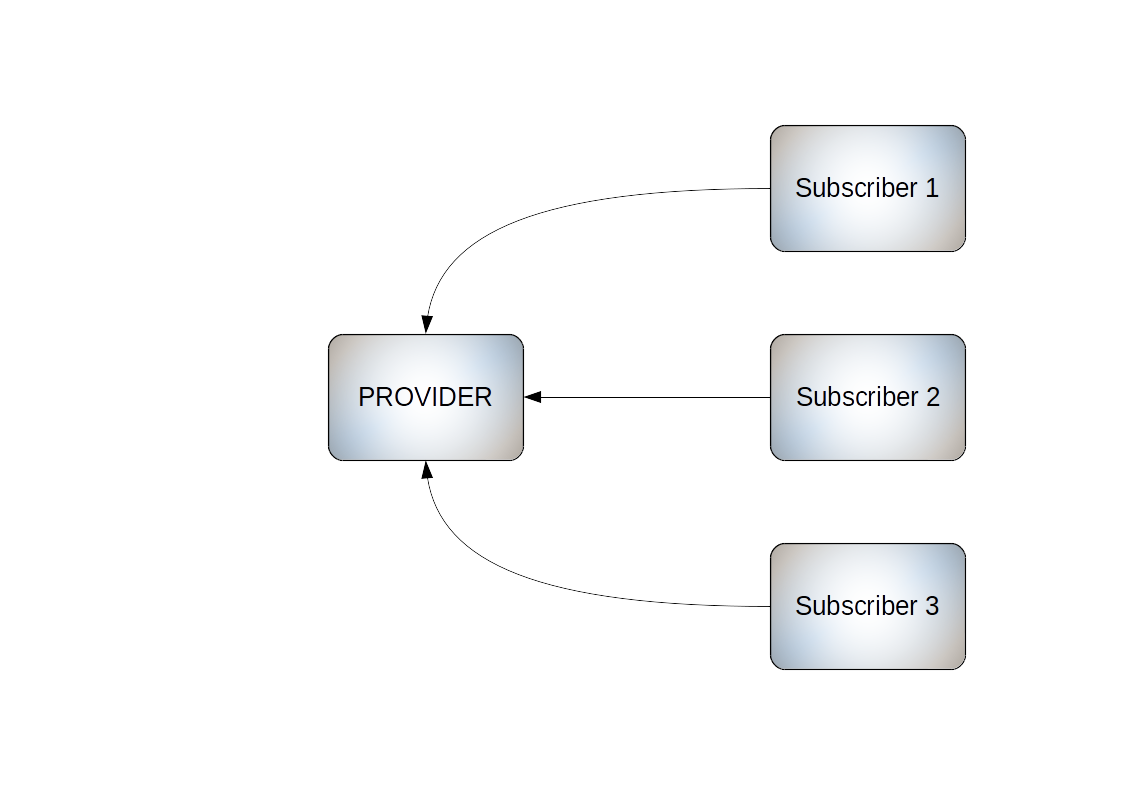
\includegraphics[scale=0.40]{img/pubsub_1.png}\\
\caption{Semplice esempio di un Provider e tre Subscriber abbonati \label{figura1.14}}
\end{figure}

Come anticipato nel capitolo precedente, la struttura base del sistema di replicazione Pglogical utilizza il modello \textit{publish/subscriber} sopra descritto.\\
Al \textit{provider} sono "abbonati" uno o pi\`{u} nodi \textit{subscribers}. Ogni nodo che riceve i dati di replica da una fonte, quindi \textit{provider}, pu\`{o} essere configurato per essere in grado di inoltrare tali dati agli altri nodi sottoscritti a s\`{e}.\\
Utilizzando la replica in cascata, ogni nodo \textit{subscriber} \`{e} in contemporanea mittente e destinatario. Pi\`{u} nello specifico, ogni sottoscrittore \`{e} anche \textit{provider} di altri \textit{subscribers}.\\ 

Ci sono tre idee distinte dietro questa capacit\`{a}:
\begin{enumerate}
\item 
La scalabilit\`{a}: un database, in particolare il \textit{publish} che riceve tutte le transazioni di aggiornamento dalle applicazioni client, ha solo una capacit\`{a} limitata di soddisfare le query dei nodi sottoscritti durante il processo di replica. 
%Per soddisfare la necessit\`{a} di un gran numero di sistemi slave di sola lettura deve essere possibile eseguire una cascata.
\item
Limitare la larghezza di banda network richiesta per un sito di backup mantenendo la possibilit\`{a} di avere pi\`{u} slave nella posizione remota.
\item
Essere in grado di configurare scenari di \textit{failover}: in una configurazione da master a slave multipli, \`{e} improbabile che tutti i nodi slave siano esattamente nello stesso stato di sincronizzazione quando il master fallisce. Per garantire che uno slave possa essere promosso al master \`{e} necessario che tutti i sistemi rimanenti possano concordare lo stato dei dati. Poich\'{e} non \`{e} possibile eseguire il \textit{rollback} di una transazione confermata, questo stato \`{e} indubbiamente lo stato di sincronizzazione pi\`{u} recente di tutti i nodi slave rimanenti.\\
\end{enumerate}

%presi da slony I - ANDRANNO BENE?

Aggiunto alle funzionalit\`{a} di PostgreSQL, che ci permette di replicare un intero database, il sistema di replicazione Pglogical pu\`{o} essere configurato per replicare in modo selettivo le righe di una tabella su entrambi i lati \textit{publisher/subscriber}.\\

Le sequenze e le tabelle sono raggruppate in modo logico dentro un set di replica (\textit{replication set}). \\
Ogni set corrisponde ai dati da replicare. \`{E} composto da una serie di flussi di dati di replica, che definiremo con $R_n$ (dove \verb"n" rappresenta la \verb"n-esimo" set di replica), contenente un gruppo di oggetti da replicare indipendenti da altri oggetti provenienti dallo stesso master. In ogni caso, tutte le tabelle che hanno relazioni che potrebbero essere espresse come vincoli di chiavi esterne e tutte le sequenze utilizzate per generare numeri di serie in queste tabelle dovrebbero essere contenute in uno stesso set.

\begin{figure}[htbp]
\centering
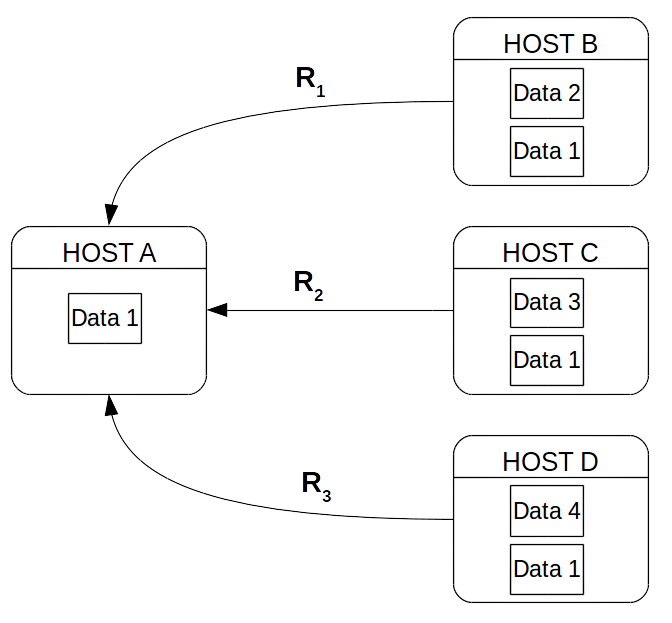
\includegraphics[scale=0.60]{img/setreplica.png}\\
\caption{Set di replica o (\textit{replication set}) \label{figura1.15}}
\end{figure}


%I parametri sono principalmente per server di invio e standby, sebbene alcuni parametri abbiano significato solo sul server master. Le impostazioni possono variare nel cluster senza problemi se necessario.


La figura illustra un semplice esempio di una configurazione di replica. Il set di replica \`{e} composto dal flusso di dati $R_1$, $R_2$ e $R_3$.
Questo scenario raffigura quattro host (nel seguente caso quattro nodi) in cui il NODO A ha il ruolo di \textit{publish} e i restanti sono i suoi sottoscrittori.
\verb"Data 1" rappresenta il flusso di dati nativi di A da replicare. Ciascun \textit{subscriber} ha esattamente i dati originali del NODO A, in quanto abbonati, in aggiunta ai propri nativi (\verb"Data 2",\verb"Data 3" e \verb"Data 4"). \\
In questo modo se il \textit{provider} fallisce (o per altri motivi non vi \`{e} pi\`{u} la possibilit\`{a} di scriverci nuovi dati), l'HOST B, in quanto suo successivo, pu\`{o} essere promosso come \textit{master} di entrambi i set.

\subsection{Simulazione di un filesystem distribuito (Dati e Metadati)}

\textbf{inserisci organizzazione mappa - per far vedere come funziona il concetto di pub/sub, range, db}
Ciascun File viene inserito dentro un \textit{bucket}, che \`{e} un insieme di record all'interno di un database, ovvero un oggetto, contenente un insieme di campi o elementi, ciascuno dei quali \`{e} identificato da un nome univoco e da un tipo di dato.\\

Di ciascun File vengono scritte due informazioni:
\begin{enumerate}
\item 
file intero diviso in chunk,
\item
una parte di metadato.
\end{enumerate}\\

\`{E} necessario replicare i metadati sulle varie \textit{Board} in modo tale che, in casi di fault, guasti o perdite, sia possibile ottenere nuovamente il dato originale.\\

Per i metadati la replica segue il concetto del modello \textit{provider/subscriber}. 
Quando \`{e} scritto un File, per ogni chunk viene fatto un calcolo di un numero \textbf{(scia e qualcosa)} combinato con un numero pseudocasuale che restituisce un ID.
Ogni Board gestisce un range di ID. \\

\textbf{figura con le board e le replication sets}

\\
Sono replicate dalle \verb"5" alle \verb"8" Board (numero gestibile da un parametro configurabile).

\\
Per quanto riguarda i dati \`{e} indispensabile scrivere i chunk.\\ 
Il dato viene splittato in due connessioni e mandato in due \textit{hosts} diversi. Pi\`{u} precisamente, \`{e} lanciata una \textit{query} in parallelo che permette la scrittura in diversi database. \\
\textbf{figura con due host e query in parallelo}

\section{Considerazioni statistiche sulla ridondanza sul dato}
\section{Considerazioni statistiche sulla ridondanza del metadato}
\section{Resilienza ai cambiamenti di rete}